%%%%%%%%%%%%%%%%% DO NOT CHANGE HERE %%%%%%%%%%%%%%%%%%%% {
    \documentclass[12pt,letterpaper]{article}
    \usepackage{fullpage}
    \usepackage[top=2cm, bottom=4.5cm, left=2.5cm, right=2.5cm]{geometry}
    \usepackage{amsmath,amsthm,amsfonts,amssymb,amscd}
    \usepackage{lastpage}
    \usepackage{enumerate}
    \usepackage{fancyhdr}
    \usepackage{mathrsfs}
    \usepackage{xcolor}
    \usepackage{graphicx}
    \usepackage{listings}
    \usepackage{hyperref}
    \definecolor{mygreen}{RGB}{28,172,0} % color values Red, Green, Blue
    \definecolor{mylilas}{RGB}{170,55,241}
    
    \hypersetup{%
      colorlinks=true,
      linkcolor=blue,
      linkbordercolor={0 0 1}
    }
    
    \setlength{\parindent}{0.0in}
    \setlength{\parskip}{0.05in}
    %%%%%%%%%%%%%%%%%%%%%%%%%%%%%%%%%%%%%%%%%%%%%%%%%%%%%%%%%% }
    
    %%%%%%%%%%%%%%%%%%%%%%%% CHANGE HERE %%%%%%%%%%%%%%%%%%%% {
    \newcommand\course{ECE 271A}
    \newcommand\semester{Fall 2019}
    \newcommand\hwnumber{\#1}                 % <-- ASSIGNMENT #
    \newcommand\NetIDa{Jiaming Lai}           % <-- YOUR NAME
    \newcommand\NetIDb{A53314574}           % <-- STUDENT ID #
    %%%%%%%%%%%%%%%%%%%%%%%%%%%%%%%%%%%%%%%%%%%%%%%%%%%%%%%%%% }
    
    %%%%%%%%%%%%%%%%% DO NOT CHANGE HERE %%%%%%%%%%%%%%%%%%%% {
    \pagestyle{fancyplain}
    \headheight 35pt
    \lhead{\NetIDa}
    \lhead{\NetIDa\\\NetIDb}                 
    \chead{\textbf{\Large Assignment \hwnumber}}
    \rhead{\course \\ \semester}
    \lfoot{}
    \cfoot{}
    \rfoot{\small\thepage}
    \headsep 1.5em
    %%%%%%%%%%%%%%%%%%%%%%%%%%%%%%%%%%%%%%%%%%%%%%%%%%%%%%%%%% }
    
    \begin{document}
     
    \section*{Computer Problem Solution}
    % If the Problem is divided into items, use "enumerate"
    \begin{enumerate}[a)]
        %%%%%%%%%%%%%%%%%%%%%%%%%%%%%%%%%%%%%%%%%%%%%%%%%%%%%%%%%%
        % Problem (a)
        %%%%%%%%%%%%%%%%%%%%%%%%%%%%%%%%%%%%%%%%%%%%%%%%%%%%%%%%%%
        \item 
        Using the training data in \textbf{TrainingSamplesDCT8.mat}, what are reasonable estimates for the prior probabilities?
        
        \textbf{Solution}:\\
        Two priors probabilities, $P_Y(cheetah)$ and $P_Y(grass)$, could be estimated based on the number of vectors in the training set.
        The estimation of $P_Y(cheetah)$ and $P_Y(grass)$ are: 
        \begin{equation}
            P_Y(cheetah) = N_{FG} / (N_{FG} + N_{BG}) = 0.1919
        \end{equation}
        \begin{equation}
            P_Y(grass) = N_{BG} / (N_{FG} + N_{BG}) = 0.8081
        \end{equation}
        where 
        \begin{itemize}
            \item[] $N_{BG}$ is the number of vectors in matrix \textbf{TrainsampleDCT\_BG}
            \item[] $N_{FG}$ is the number of vectors in matrix \textbf{TrainsampleDCT\_FG}
        \end{itemize}
        
        %%%%%%%%%%%%%%%%%%%%%%%%%%%%%%%%%%%%%%%%%%%%%%%%%%%%%%%%%%
        % Problem (b)
        %%%%%%%%%%%%%%%%%%%%%%%%%%%%%%%%%%%%%%%%%%%%%%%%%%%%%%%%%%
        \item 
        Using the training data in \textbf{TrainingSamplesDCT8.mat}, compute and plot the index histograms
        $P_{X|Y}(x|cheetah)$ and $P_{X|Y}(x|grass)$. 
        
        \textbf{Solution}:\\
        According to training data, the frequency histograms is the following picture:
        \begin{figure}[h]
            \centering
            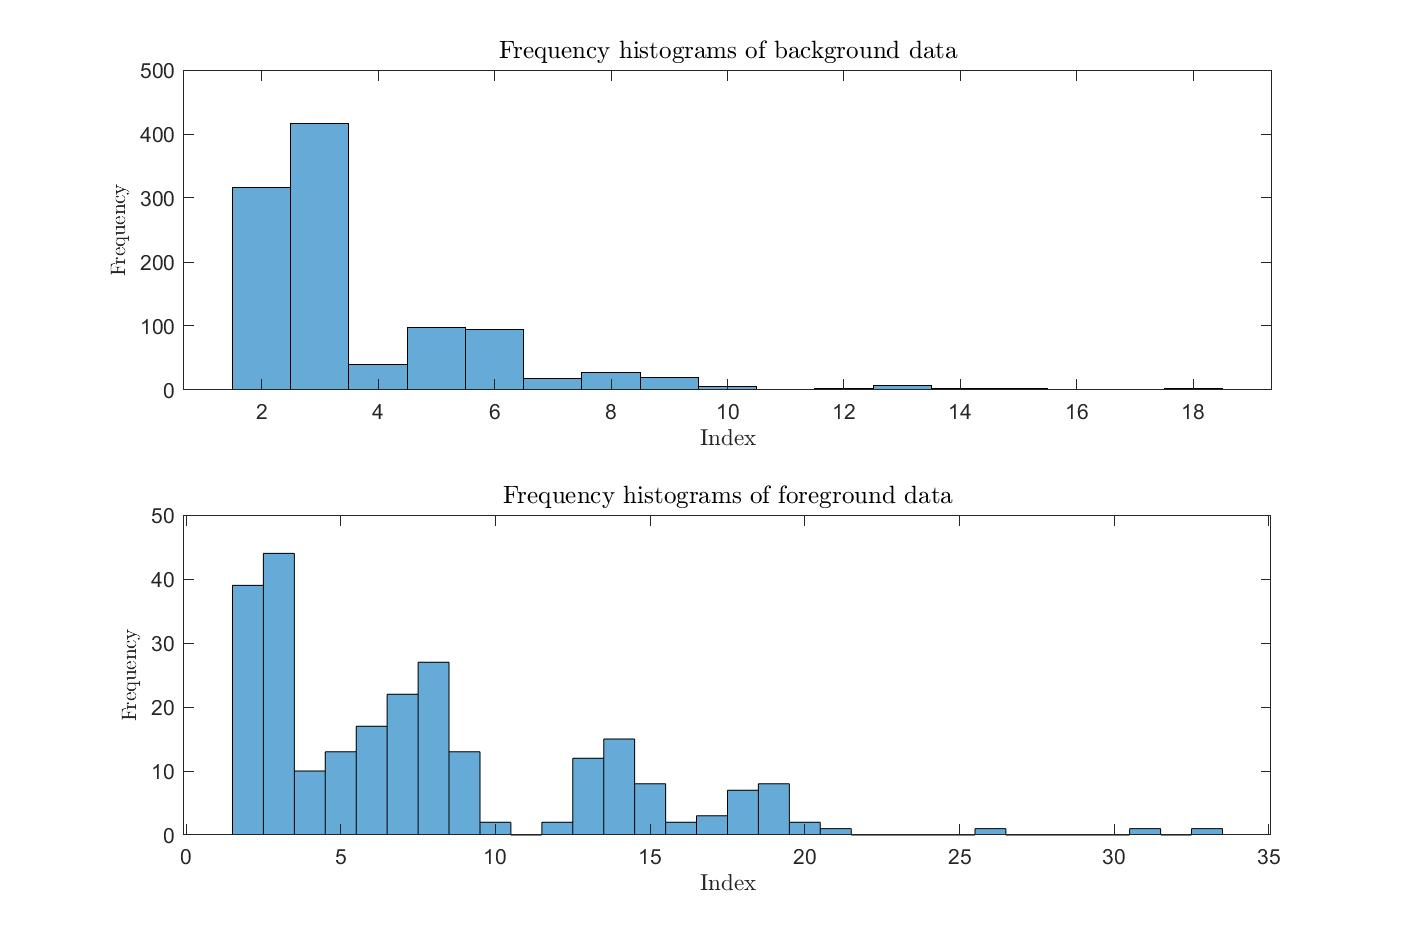
\includegraphics[scale=0.2]{Images/histograms1.jpg}
            \caption{Frequency histograms}
        \end{figure}\\
        \\
        \\
        The index histograms of $P_{X|Y}(x|cheetah)$ and $P_{X|Y}(x|grass)$ is showed as following:
        \begin{figure}[h]
            \centering
            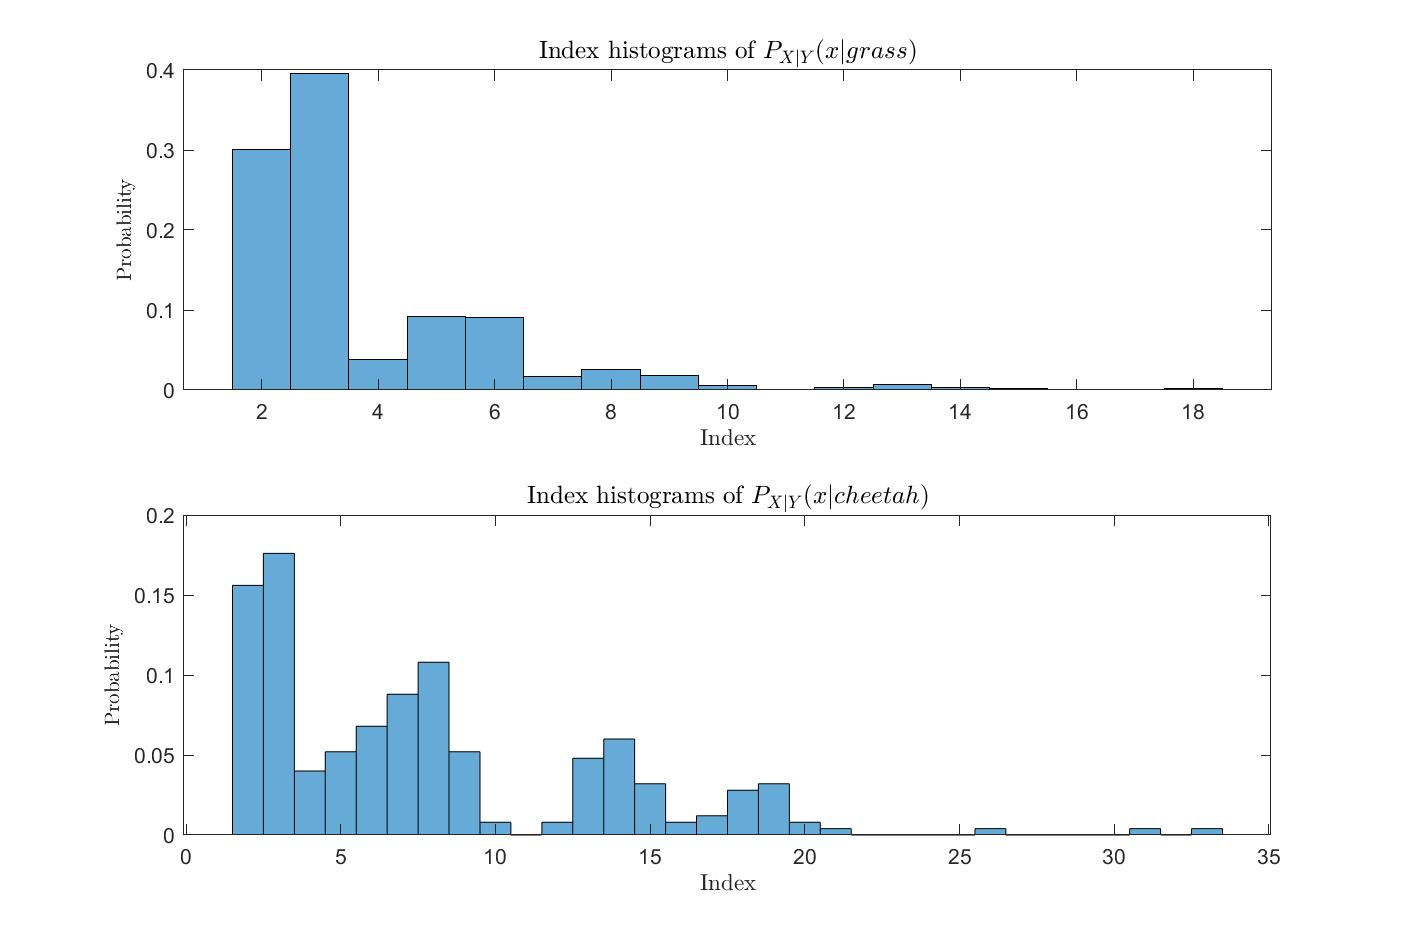
\includegraphics[scale=0.2]{Images/histograms2.jpg}
            \caption{Index histograms}
        \end{figure}

        %%%%%%%%%%%%%%%%%%%%%%%%%%%%%%%%%%%%%%%%%%%%%%%%%%%%%%%%%%
        % Problem (c)
        %%%%%%%%%%%%%%%%%%%%%%%%%%%%%%%%%%%%%%%%%%%%%%%%%%%%%%%%%%
        \item    
        For each block in the image \textbf{cheetah.bmp}, compute the feature X (index of the DCT coefficient with $2^{nd}$ greatest energy).
        Compute the state variable Y using the minimum probability of error rule based on the probabilities obtained in a) and b).
        Store the state in an array A. Using the commands imagesc and colormap(gray(255)) create a picture of that array.
        
        \textbf{Solution}:\\
        Given a 8*8 block from the image \textbf{cheetah.bmp}, we can easily compute an array of 8*8 frequency coefficients by using
        funcition \textbf{dct2} on Matlab. Feature X would be index of the $2^{nd}$ greatest DCT coefficient. Given $X=x$ in one block,
        according to the minimum probability of error rule, we can pick state of cheetah if:
        \begin{equation}
            \frac{P_{X|Y}(x|cheetah)}{P_{X|Y}(x|grass)} > T = \frac{P_Y(grass)}{P_Y(cheetah)}
        \end{equation}
        where 
        \begin{itemize}
            \item[] $P_{X|Y}(x|cheetah)$ and $P_{X|Y}(x|grass)$ are the estimation we get from training data.
            \item[] $P_Y(cheetah)$ and $P_Y(grass)$ are the estimation we get from training data.
            \item[] $T$ is the threshold.
        \end{itemize}
        Then we mask the top left corner of the 8*8 block as 1, regarding this pixel belongs to cheetah.
        Otherwise, we mask 0. By using a sliding window that moves by one pixel at each step, finally we get a array A containing the mask indicates 
        which blocks contain grass and which contain the cheetah.

        %%%%%%%%%%%%%%%%%%%%%%%%%%%%%%%%%%%%%%%%%%%%%%%%%%%%%%%%%%
        % Problem (d)
        %%%%%%%%%%%%%%%%%%%%%%%%%%%%%%%%%%%%%%%%%%%%%%%%%%%%%%%%%%
        \item  
        The array A contains a mask that indicates which blocks contain grass and which contain the cheetah. Compare it with the ground
        truth provided in image \textbf{cheetah mask.bmp} (shown below on the right) and compute the probability of error of your algorithm.
        
        \textbf{Solution}:\\
        The comparision between ground truth and picture generated from array A is showed as following:
        \begin{figure}[h]
            \centering
            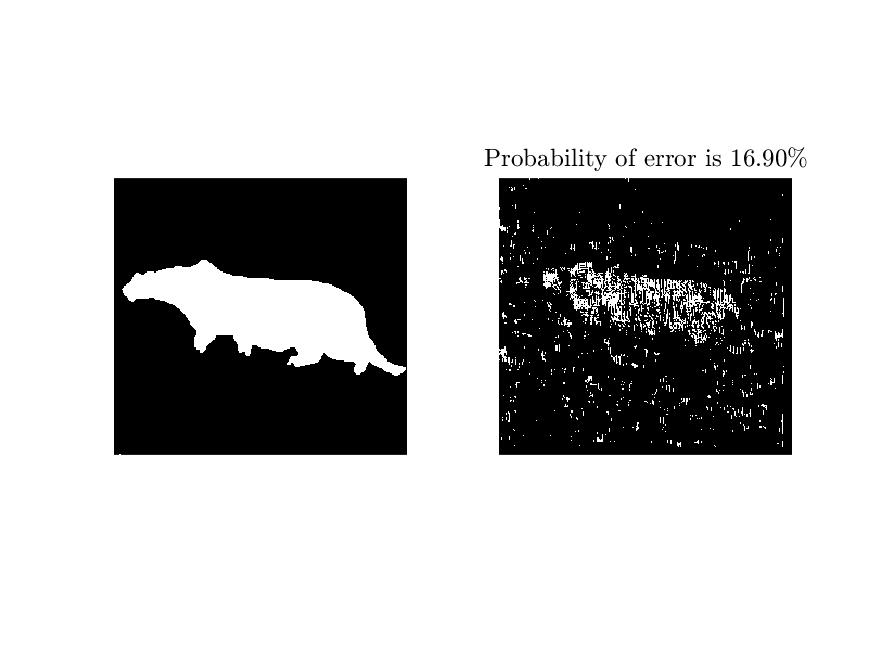
\includegraphics[scale=0.4]{Images/segmentation.jpg}
            \caption{Comparision}
        \end{figure}\\
        The probabilities of error is 16.90\%, as showed in the figure above.
    \end{enumerate}

    \section*{Appendix}
    The following is the Matlab code.
    \lstset{language=Matlab,%
        %basicstyle=\color{red},
        breaklines=true,%
        morekeywords={matlab2tikz},
        keywordstyle=\color{blue},%
        morekeywords=[2]{1}, keywordstyle=[2]{\color{black}},
        identifierstyle=\color{black},%
        stringstyle=\color{mylilas},
        commentstyle=\color{mygreen},%
        showstringspaces=false,%without this there will be a symbol in the places where there is a space
        numbers=left,%
        numberstyle={\tiny \color{black}},% size of the numbers
        numbersep=9pt, % this defines how far the numbers are from the text
        emph=[1]{for,end,break},emphstyle=[1]\color{red}, %some words to emphasise
        %emph=[2]{word1,word2}, emphstyle=[2]{style},    
    }
    \lstinputlisting{HW1_solution.m}

    \end{document}